\XtoCBlock{Create Documentation}
\label{block:CreateDocumentation}
\begin{figure}[H]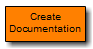
\includegraphics{CreateDocumentation}\end{figure} 

\subsubsection*{Description:}
This system block is used to generate a documentation of the current project. The document will be created in \textit{X2CCode\textbackslash ..\textbackslash Documentation} and will be called \textit{ProjectDocumentation_<Name of model>.pdf}.

\subsubsection*{Parameters}
\paragraph*{Test reports:}
If the checkbox \textit{Add test reports} is selected, test reports of the C-Unit tests of the used X2C blocks are added to the project documentation.

\paragraph*{User documentation:}
The user has the possibility to add user specific documentation to the project documentation. When creating the project documentation, the \textit{X2CCode} directory is scanned for a \textit{UserDoc.tex} file. If this file is present, it will be included in the documentation.

\subsubsection*{Requirements}
In order to generate a documentation in PDF-format a TeX-compiler (e.g. MiKTeX) has to be installed.


